\documentclass[11pt]{article}
\usepackage[margin=2cm]{geometry}
\usepackage{graphicx}
\usepackage{amsmath,amssymb}
\setlength{\parindent}{0pt}\setlength{\parskip}{5pt}
\newcommand{\code}[1]{\texttt{#1}}
\graphicspath{{figures/}}
\begin{document}
\begin{center}{\Large\bfseries s9\_tarc --- Figure Notes for the Defense}\\[2pt]
s9 direct-velocity whole-body (14/8), T-arc curriculum. Gate 0.02~m / 1.15$^\circ$; 100\% reached; mean min $d$ 13.2~mm, mean min $\varphi$ 0.39$^\circ$, mean 83 decisions (8.3~s) to the gate. Checkpoint ppo\_scoutsan\_s9\_tarc.zip, 2026-09-25.\end{center}
\vspace{4pt}
\section*{Figure 1 --- Reach: distance to target}
\begin{center}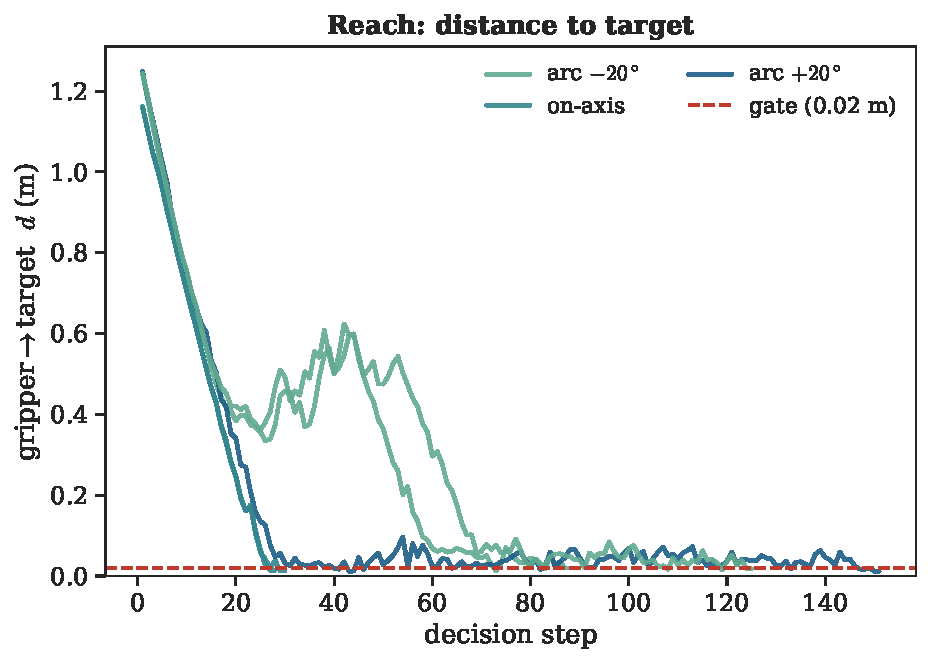
\includegraphics[width=0.8\textwidth,height=0.55\textheight,keepaspectratio]{s9tarc_reach.pdf}\end{center}
\textbf{What it shows.} Gripper$\to$target distance $d$ vs decision step, one curve per pass, coloured by WHICH of the three curriculum targets it is (arc $-20^\circ$ / on-axis / arc $+20^\circ$); red dashed = the 0.02~m position gate.

\textbf{How to read it.} Every pass converges under the gate (reached rate 100\%). The curve stops at the gate because the agent ends the episode there.

\textbf{Say this.} ``All 5 passes reach the 0.02~m gate, mean minimum distance 13.2~mm.''

\textbf{If asked.} \emph{Why do the curves end at different lengths?} --- each curve ends when its target is reached; the on-axis target is far quicker than the $\pm20^\circ$ arc ones.
\clearpage
\section*{Figure 2 --- Confondu: orientation error}
\begin{center}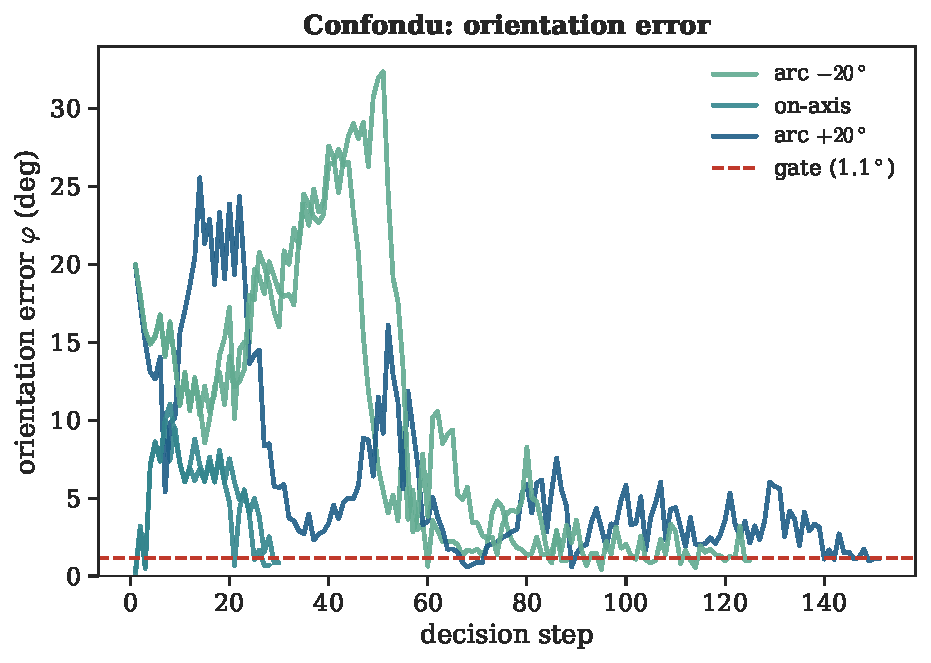
\includegraphics[width=0.8\textwidth,height=0.55\textheight,keepaspectratio]{s9tarc_orient.pdf}\end{center}
\textbf{What it shows.} Orientation error $\varphi$ (deg) vs step; gate = 1.15$^\circ$ (0.02~rad). $\varphi = 2\arccos|\langle q_G,q_T\rangle|$, the geodesic angle between the gripper and target frames.

\textbf{How to read it.} $\varphi$ starts near $90^\circ$ (the gripper faces its home pose, the target faces away from the robot) and falls under the gate together with the distance --- that simultaneity is what \emph{confondu} means.

\textbf{Say this.} ``Orientation converges to a mean minimum of 0.39$^\circ$, under the 1.15$^\circ$ gate.''

\textbf{If asked.} \emph{Why is position alone not enough?} --- the task is frame coincidence: the gripper must arrive with the right orientation, not just at the right point.
\clearpage
\section*{Figure 3 --- Base drives into arm reach}
\begin{center}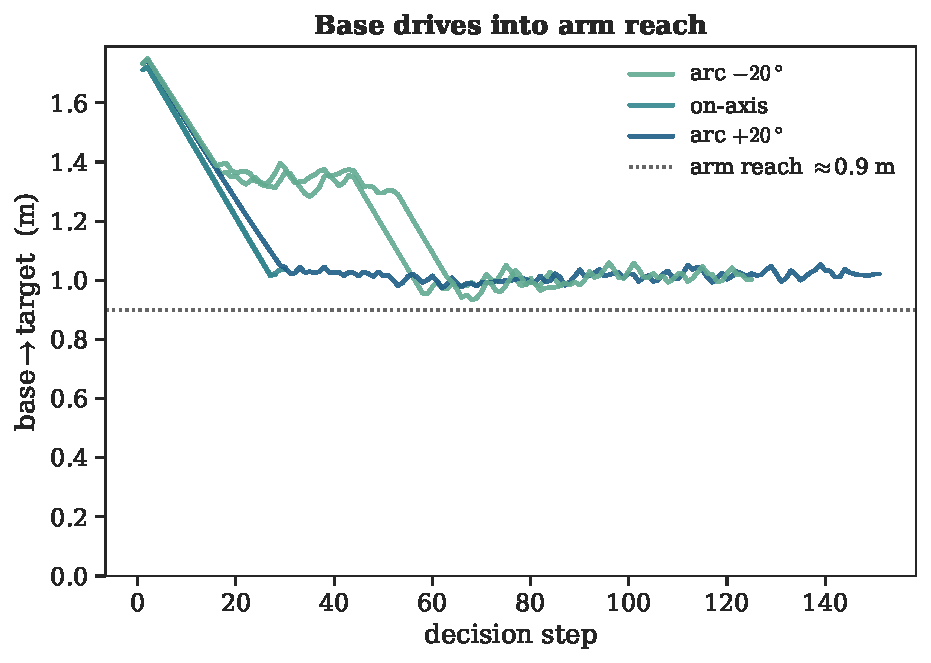
\includegraphics[width=0.8\textwidth,height=0.55\textheight,keepaspectratio]{s9tarc_basedrive.pdf}\end{center}
\textbf{What it shows.} base\_link$\to$target distance vs step --- the mobile base's contribution, separated from the arm's. The dotted line marks the $\approx$0.9~m arm reach.

\textbf{How to read it.} The base closes from about 2~m to inside arm reach and then holds while the arm finishes; this is the whole-body split the single policy learned on its own (no hand-coded hand-off).

\textbf{Say this.} ``One policy drives the base AND the arm: the base brings the target inside the arm's reach, then the arm performs the alignment.''

\textbf{If asked.} \emph{Is the split hand-coded?} --- no: the 8 actions are 6 joint deltas plus base $v,\omega$; the division of labour is learned.
\clearpage
\section*{Figure 4 --- Joint convergence into the gate corner}
\begin{center}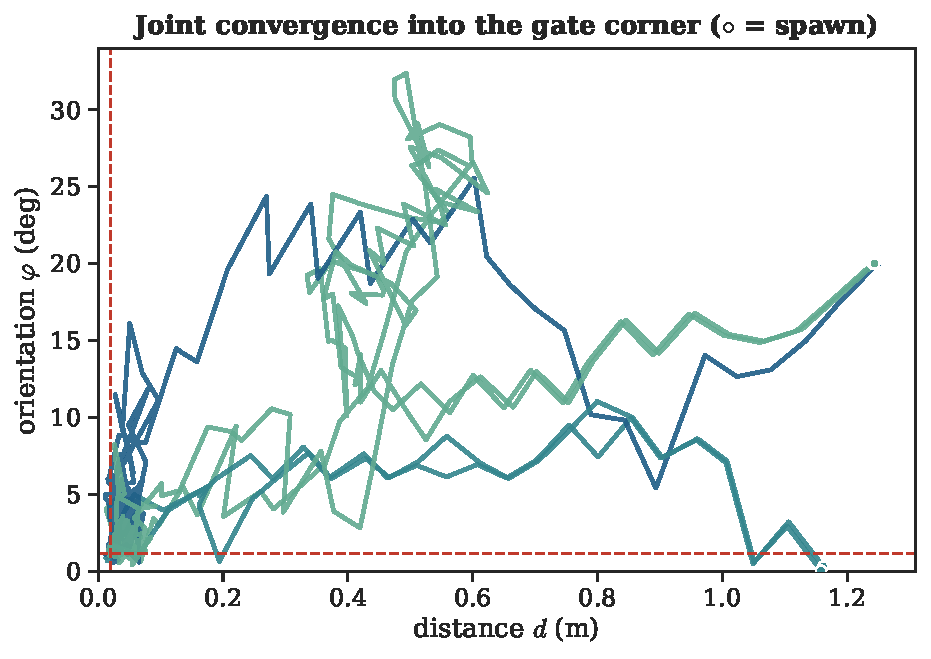
\includegraphics[width=0.8\textwidth,height=0.55\textheight,keepaspectratio]{s9tarc_phase.pdf}\end{center}
\textbf{What it shows.} $\varphi$ plotted against $d$ (a phase portrait); the open circle is the spawn, the red lines are the two gate thresholds. The bottom-left corner is \emph{confondu}.

\textbf{How to read it.} The trajectories sweep down-left into the corner instead of hugging one axis --- position and orientation are reduced together, not one after the other.

\textbf{Say this.} ``Both errors enter the gate corner together --- the policy does not trade position for orientation.''

\textbf{If asked.} \emph{What would a bad policy look like?} --- a curve that runs down the $d$ axis first and only then drops in $\varphi$ (reach, then fix the wrist), which wastes time and often stalls.
\clearpage
\section*{Figure 5 --- Speed per target}
\begin{center}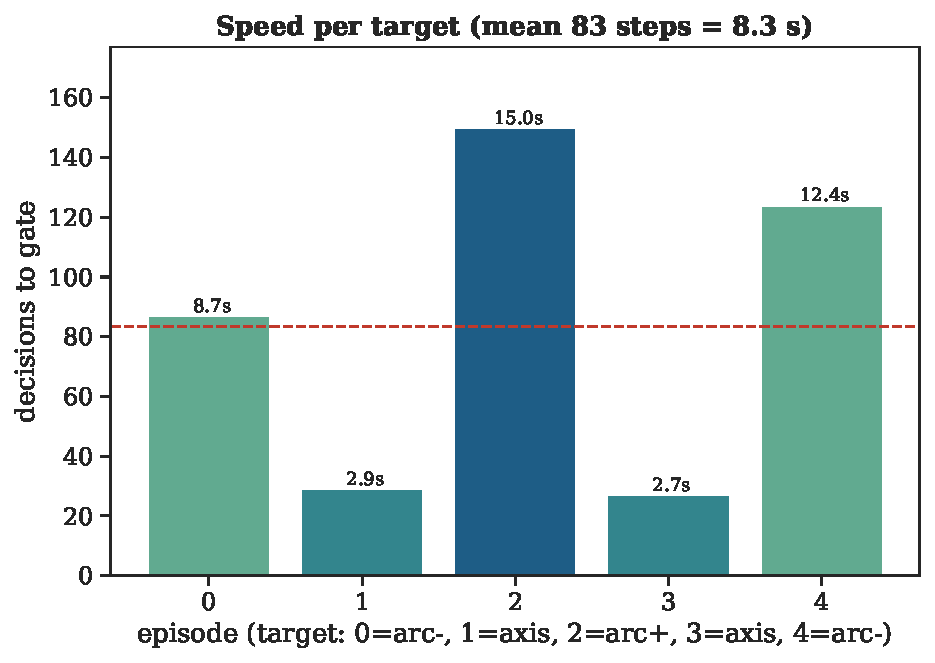
\includegraphics[width=0.8\textwidth,height=0.55\textheight,keepaspectratio]{s9tarc_speed.pdf}\end{center}
\textbf{What it shows.} Decisions to first enter the gate, per pass, annotated in seconds (1 decision = 0.1~s).

\textbf{How to read it.} Mean 83 decisions = 8.3~s. The on-axis target is reached in a fraction of the time the arc targets need.

\textbf{Say this.} ``Mean 8.3~s to the gate over the sweep.''

\textbf{If asked.} \emph{Comparable to the WDLS regimes?} --- yes: same three targets, same gate, same 0.1~s decision period. See \code{comparison\_speed.pdf} at the top of \code{deliverables/}.
\clearpage
\section*{Figure 6 --- Trajectories in the target frame}
\begin{center}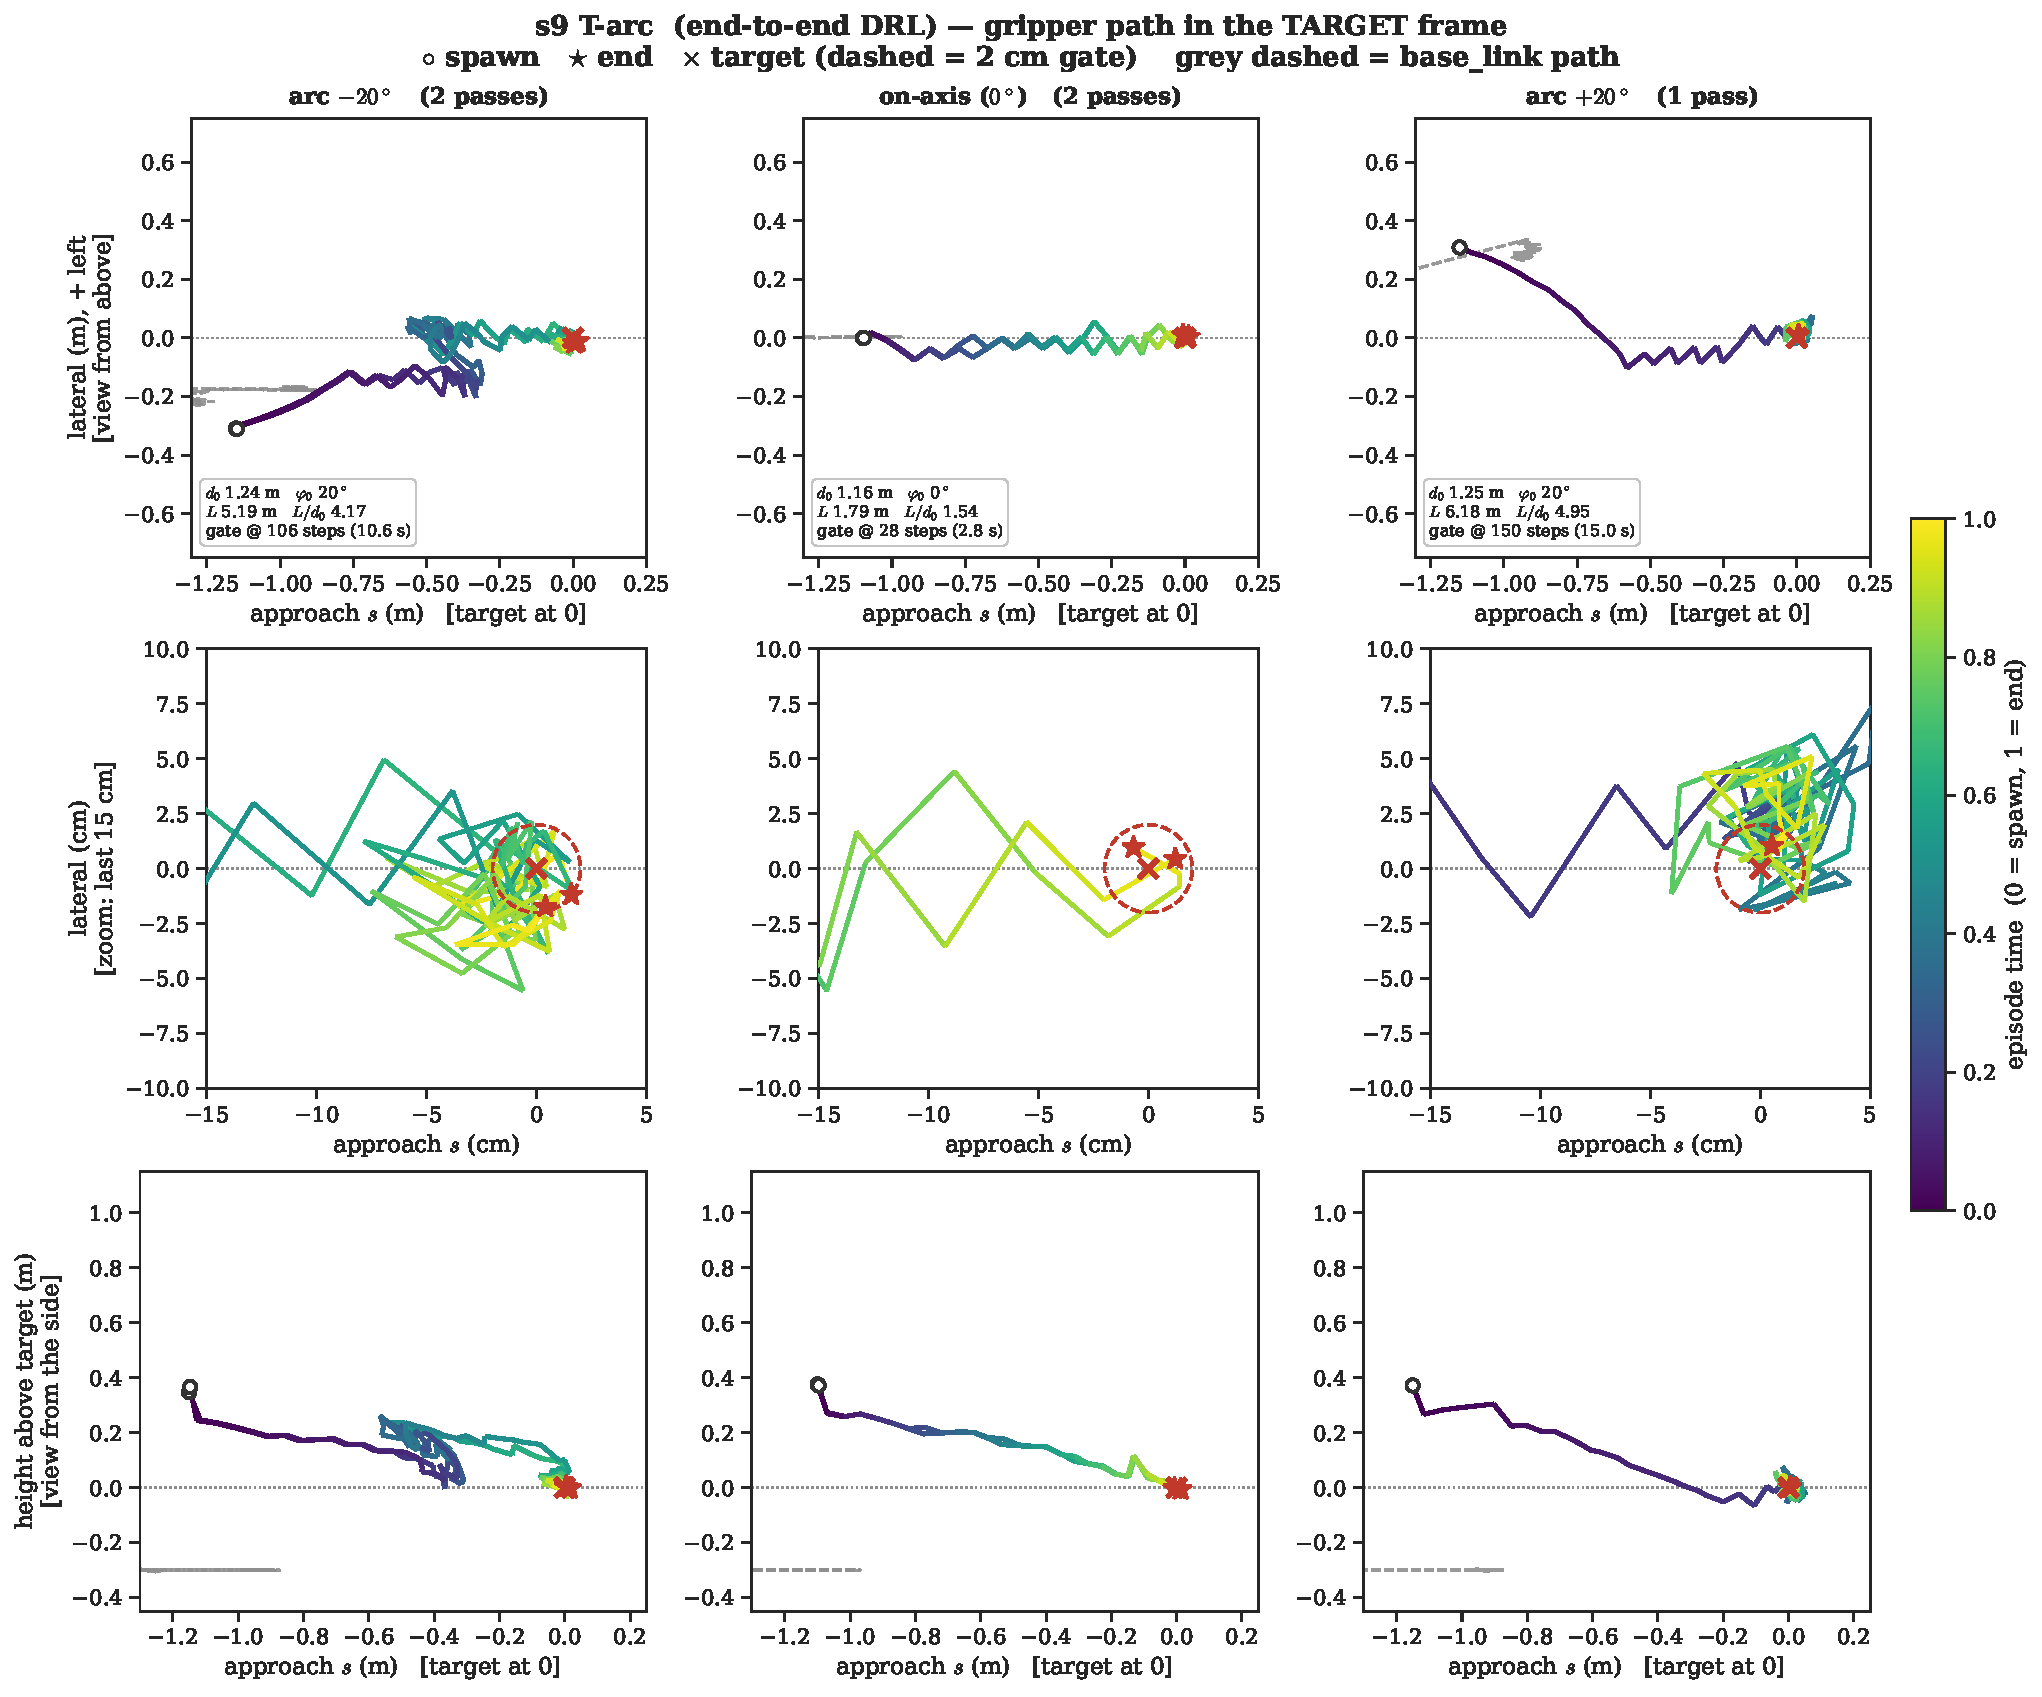
\includegraphics[width=0.99\textwidth,height=0.66\textheight,keepaspectratio]{trajectories.pdf}\end{center}
\textbf{What it shows.} The gripper's path expressed in the TARGET's own frame: $s$ = approach coordinate along the target's outward axis (the robot starts at $s<0$, the target is $s=0$), lateral = sideways offset, height = above the target. Colour = time within the episode. One column per curriculum target.

\textbf{How to read it.} Mean path length is 3.28$\times$ the straight-line distance, with up to 31~cm of lateral excursion on the arc targets; the zoom row shows the last 15~cm entering the 2~cm gate. The grey dashed line is where the BASE went --- the base covers the long haul, the arm does the final alignment.

\textbf{Say this.} ``Drawn in the target frame, the path is directly comparable with the other controllers --- same targets, same axes, so the shapes can be read side by side.''

\textbf{If asked.} \emph{Why the target frame?} --- the gripper$\to$target relative pose is frame-independent, so it does not matter that the end-to-end model observes in base\_link FLU while the WDLS logs are in Unity world coordinates. It is the only frame in which the two are comparable.
\clearpage
\section*{Figure 7 --- Overview (one-slide summary)}
\begin{center}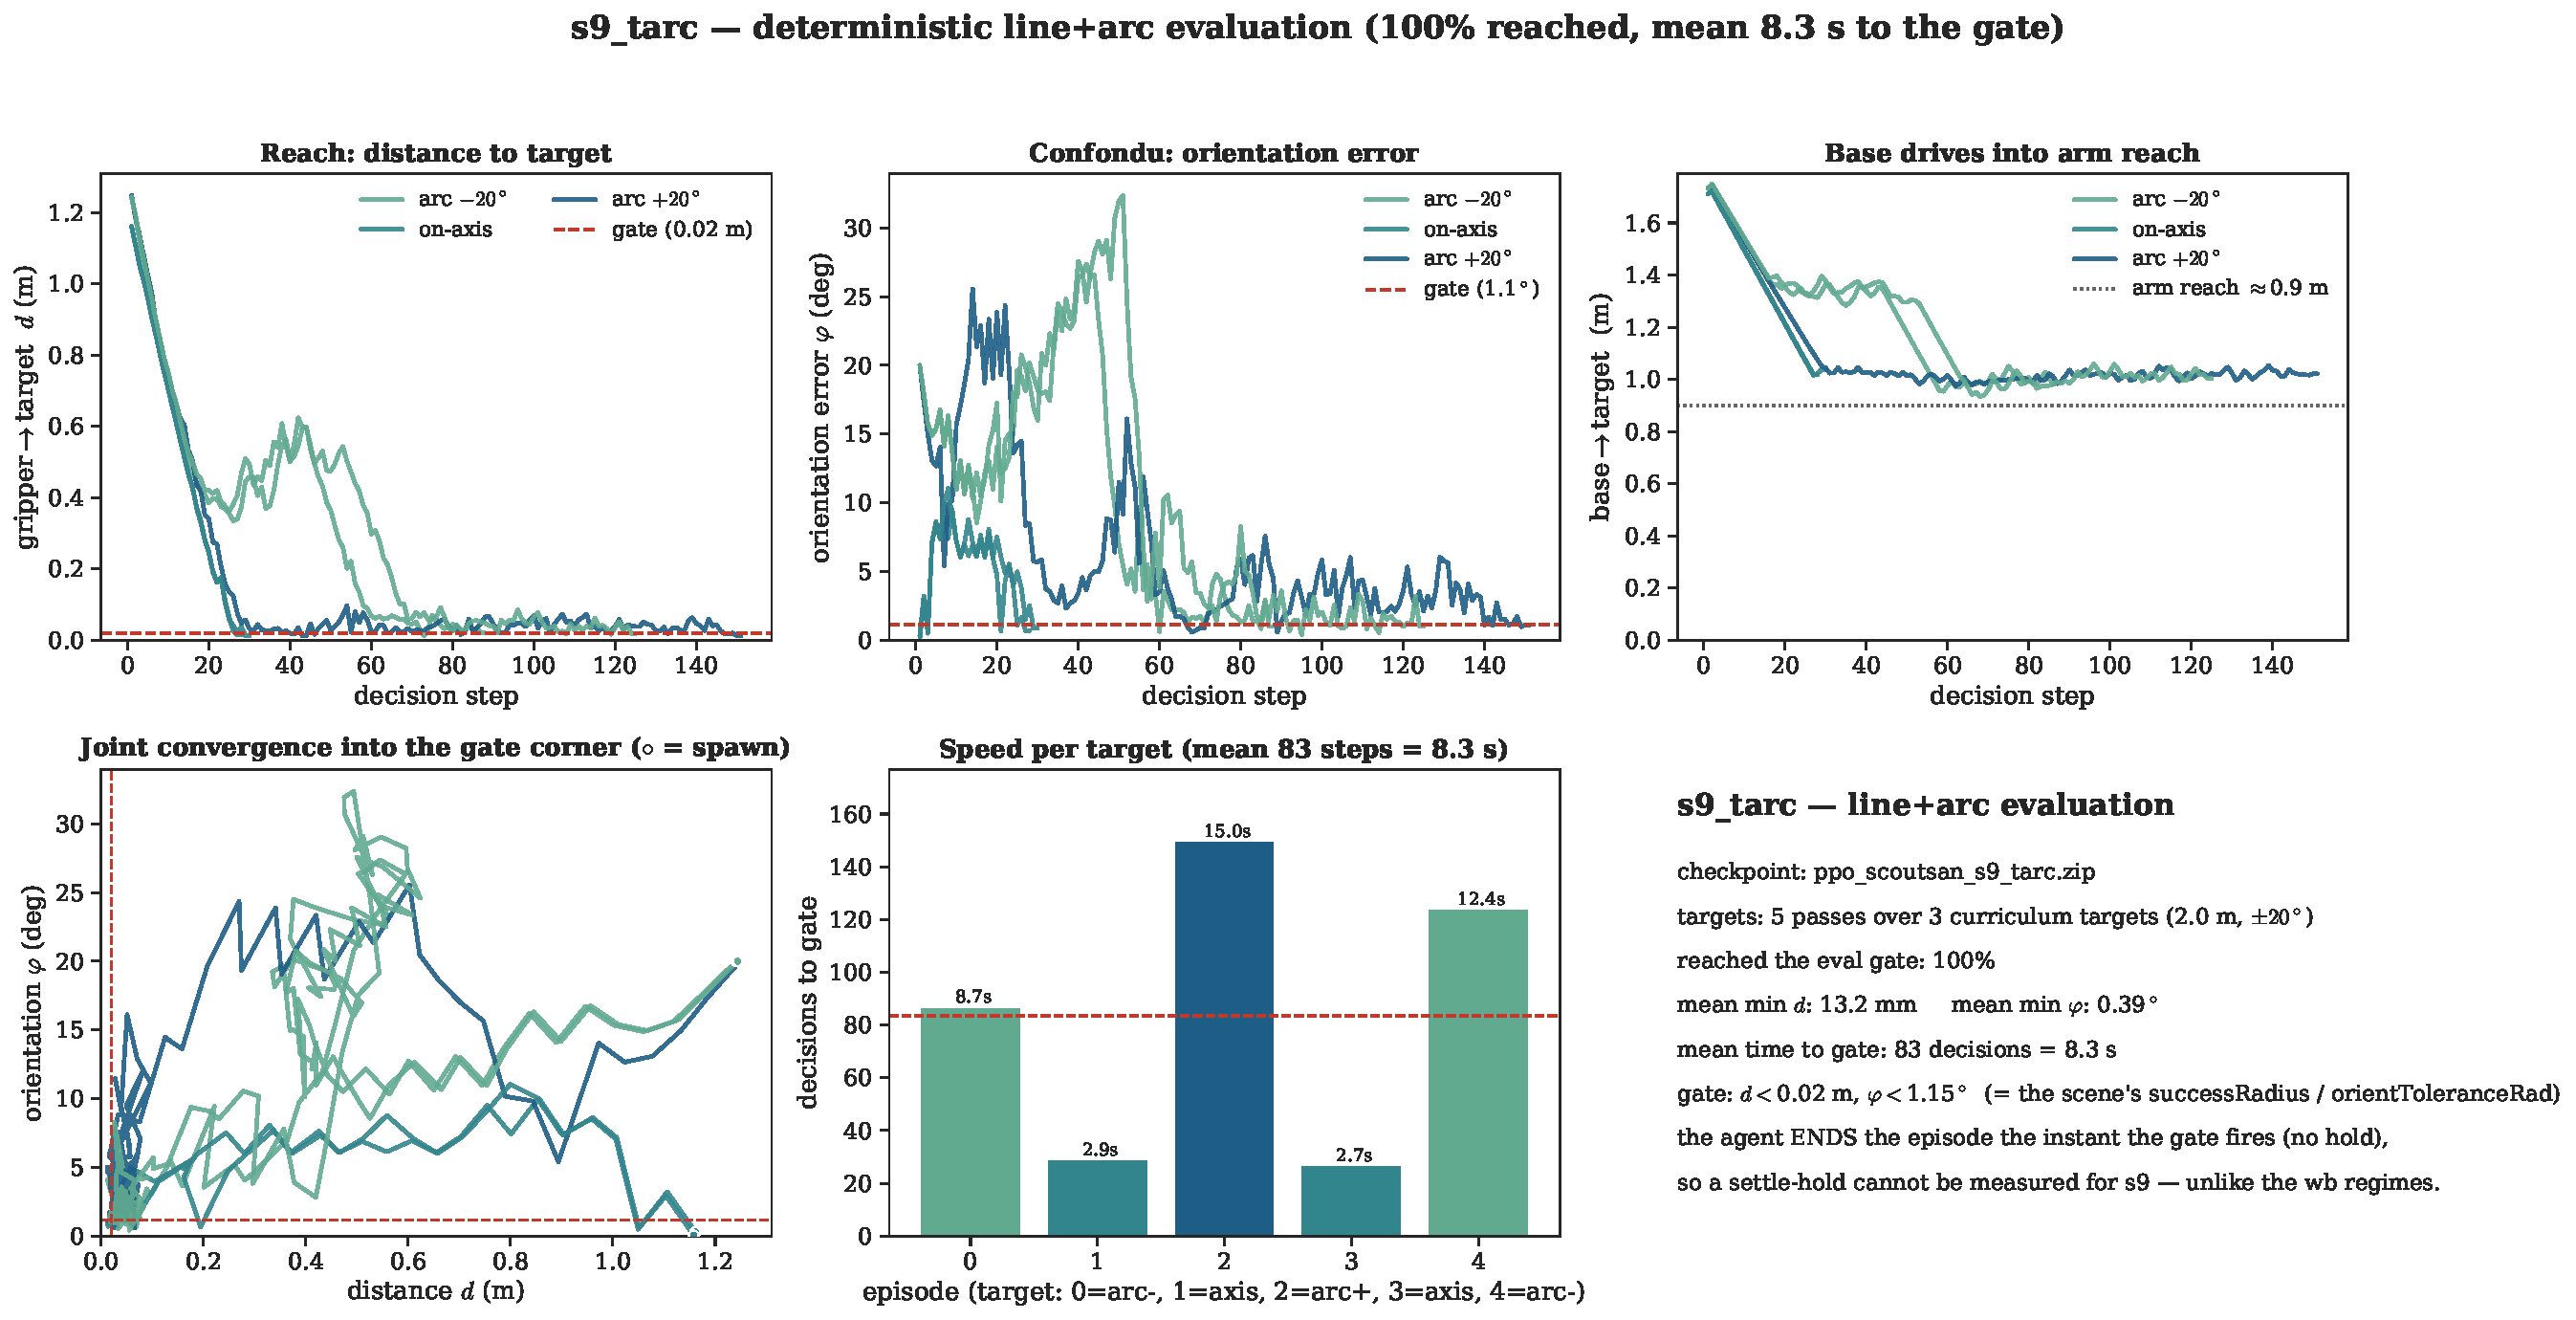
\includegraphics[width=0.8\textwidth,height=0.55\textheight,keepaspectratio]{s9tarc_overview.pdf}\end{center}
\textbf{What it shows.} Reach, orientation, base drive, phase portrait and per-target speed on one figure, plus the numbers.

\textbf{How to read it.} Use as the summary slide; the panels are detailed on the preceding pages.

\textbf{Say this.} ``s9\_tarc: 100\% of the sweep reached, mean min $d$ 13.2~mm, mean min $\varphi$ 0.39$^\circ$, 8.3~s to the gate.''

\textbf{If asked.} \emph{What does T-arc add over the fixed-target s9?} --- the same agent and reward, trained on a curriculum that grows the target from close and on-axis out to 2~m and $\pm20^\circ$; this eval is the whole sweep, not a single pose.
\clearpage
\end{document}
